\documentclass[13pt]{extarticle}
\usepackage{pdfpages}
\usepackage[a4paper,pdftex]{geometry}	
\usepackage{listings}
\usepackage{xcolor}
\usepackage{fix-cm}
\usepackage[russian]{babel}
\usepackage[utf8]{inputenc}
\usepackage{mathtools}
\usepackage{tabularx}
% Using typewriter font: \ttfamily inside \lstset

\lstset{language=C++,
                basicstyle=\ttfamily,
                keywordstyle=\color{blue}\ttfamily,
                stringstyle=\color{red}\ttfamily,
                commentstyle=\color{green}\ttfamily,
                morecomment=[l][\color{magenta}]{\#}
}


%Images
\usepackage{graphicx}
\DeclareGraphicsExtensions{.pdf,.png,.jpg}
\usepackage{wrapfig}
\renewcommand{\thefigure}{\thesection.\arabic{figure}}
\renewcommand{\thetable}{\thesection.\arabic{figure}}


\geometry{top=2cm} % отступ сверху
\geometry{bottom=2.5cm} % отступ снизу
\geometry{left=2cm} % отступ справа
\geometry{right=2cm}


\author{Пахтусов Н. Г., ПРО-306}
\makeatletter

%Roman num
\newcommand*{\rom}[1]{\expandafter\@slowromancap\romannumeral #1@}


\begin{document}

\begin{center}
\thispagestyle{empty} 

Федеральное государственное бюджетное образовательное учереждение высшего \\
профессионального образования\\
<<Уфимский государственный авиационный технический университет>>
\vspace*{\fill}
\begingroup
\centering

Отчёт по лабораторной работе №1\\
по дисциплине <<Компьютерная графика>>\\
<<Точка в 3D пространстве>>

\endgroup
\vspace*{\fill}

\end{center}

\begin{flushright}

Выполнил:\\
\@author \\
Проверил: \\
Верхотуров М. А.

\end{flushright}

\begin{center}
$\bullet$ Уфа, 2015
\end{center}

\clearpage

\tableofcontents

\clearpage

\section{Постановка задачи}
\subsection{Содержательная постановка задачи}
	Содержание экрана:
	\begin{itemize}
		\item пространственный чертеж с изображением точки Т, ее проекций Т$_1$, Т$_2$, Т$_3$ и линий связи;
		\item  комплексный чертеж с изображением проекций Т$_1$, Т$_2$, Т$_3$ и линий связи.
		\item ползунковые переключатели для интерактивного изменения координат (x, y, z) точки Т и угла $\alpha$.
	\end{itemize}
	Динамика:
	\begin{itemize}
		\item при изменении координат точки Т и угла $\alpha$, должны изменяться соответствующие проекции и сама точка Т на пространственном и комплексном чертежах.
	\end{itemize}
\subsection{Формальная постановка задачи}
	\begin{figure}[h]
		\center{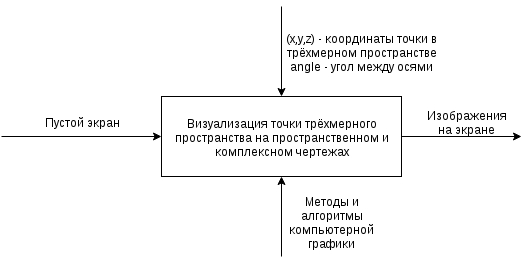
\includegraphics{Images/frst}}
		%\caption{Формальная постановка задачи.}
	\end{figure}
	
\section{Теоретическая часть}
\subsection{Ортогональная система трех плоскостей проекций}
В основу построения любого изображения положена операция проецирования.

Сущность метода ортогонального проецирования заключается в том, что предмет проецируется на две взаимно перпендикулярные плоскости лучами, ортогональными (перпендикулярными) к этим осям.

Одну из плоскостей проекций П$_1$ располагают горизонтально, а вторую, П$_2$, -- вертикально. Плоскость П$_1$ называют горизонтальной плоскостью проекций, П$_2$ -- фронтальной. Плоскости П$_1$ и П$_2$ бесконечны и непрозрачны.

При построении проекций необходимо помнить, что проекцией точки на плоскость называется основание перпендикуляра, опущенного из этой точки на данную плоскость. Проекцию точки А на горизонтальную плоскость называют горизонтальной проекцией и обозначают А$_1$, проекцию точки А на фронтальную плоскость -- фронтальной проекцией и обозначают А$_2$. Каждая из них является основанием перпендикуляра, опущенного из данной точки А соответственно и на плоскости П$_1$ и П$_2$. Две проекции точки определяют её положение в пространстве. Так как каждая фигура или тело представляет собой совокупность точек, можно утверждать, что две ортогональные проекции предмета (при наличии буквенных обозначений) вполне определяют его форму.

Однако, в практике изображения строительных конструкций, машин и различных инженерных сооружений возникает необходимость в создании дополнительных проекций. Чтобы сделать проекционный чертеж более ясным и удобочитаемым, используют третью плоскость, перпендикулярную П$_1$ и П$_2$. Эта плоскость обозначается буквой П$_3$  и называется профильной.

Проекции точек на плоскость П$_3$ называются профильными и обозначают А$_3$.

	\begin{wrapfigure}[21]{r!}{0.5\linewidth}
		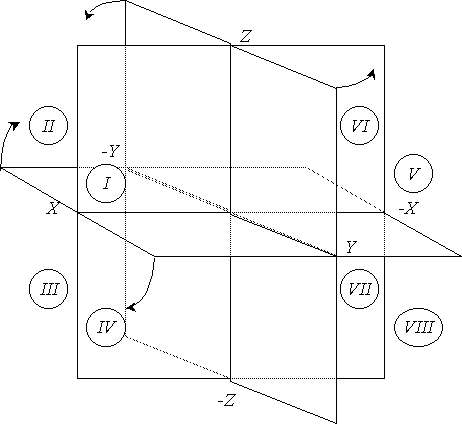
\includegraphics[width=0.48\textwidth]{Images/ortogonalSystem}
		\caption{Ортогональная система плоскостей.}
		\label{fig:ortSys}
	\end{wrapfigure}
	Плоскости проекций, попарно пересекаясь, определяют три оси: O$_x$, O$_y$ и O$_z$, которые можно рассматривать как систему прямоугольных декартовых координат в пространстве с началом в точке O. Система знаков, соответствующая <<правой системе>> координат, показана на Рис. \ref{fig:ortSys}.

Три плоскости проекций делят пространство на восемь трехгранных углов -- это так называемые октанты. Нумерация октантов дана на Рис. \ref{fig:ortSys}.

Рассматривая ортогональные проекции, предполагают, что наблюдатель находится в первом октанте. Проекционный чертеж, на котором плоскости проекций со всем тем, что на них изображено, совмещены особым образом одна с другой, называется эпюром. Для получения эпюра плоскости П$_1$ и П$_3$ вращают как показано на Рис. \ref{fig:ortSys} до совмещения с плоскостью П$_2$. В результате вращения передняя полуплоскость П$_1$ оказывается совмещенной с нижней полуплоскостью П$_2$, а задняя полуплоскость П$_1$ -- с верхней полуплоскостью П$_2$.

	\begin{wrapfigure}[14]{h}{\linewidth} 
		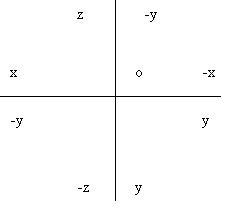
\includegraphics[width=0.48\textwidth]{Images/complexDraw}
		\caption{Вид совмещённых плоскостей.}
		\label{fig:complDr}
	
	\end{wrapfigure}

	Окончательный вид всех совмещенных плоскостей проекций дан на Рис. \ref{fig:complDr}

\subsection{Три координаты и три проекции точки}
\emph{Координатами} называют числа, которые ставят в соответствие точке для определения ее положения в пространстве или на поверхности.
В трехмерном пространстве положение точки устанавливают с помощью прямоугольных декартовых координат (x, y, z). Абсцисса X определяет расстояние от данной точки до плоскости П$_3$, ордината Y -- до плоскости П$_2$ и аппликата Z -- до плоскости П$_1$. Приняв для отсчета координат точки систему, показанную на Рис. \ref{fig:ortSys} , составим таблицу знаков координат во всех восьми октантах (см. таблицу).
	\begin{tabular}{ |c|c|c|c| }
		\hline
	  	Октант & \multicolumn{3}{ |c| }{Знаки координат} \\
	  	\cline{2-4}
	  	& x & y & z\\
	  	\hline
 		 \rom{1} & + & + & +\\
 	  	\hline
 		 \rom{2} & + & -- & +\\
 		\hline
 		 \rom{3} & + & -- & --\\
 		 \hline
 		 \rom{4} & + & + & --\\	
 		 \hline
 		 \rom{5} & - & + & +\\	
 		 \hline
 		 \rom{6} & -- & -- & +\\	
 		 \hline
 		 \rom{7} & -- & -- & --\\	
 		 \hline
 		 \rom{8} & -- & + & --\\	
 		 \hline	 
\end{tabular}

Какая-либо точка пространства A, заданная координатами, будет обозначаться так: A (x, y, z). Построение изображения самой точки и ее проекций на пространственной модели рекомендуется осуществлять с помощью координатного прямоугольного параллелепипеда. Прежде всего, на осях координат от точки O откладывают отрезки, соответственно равные единицам длины. На этих отрезках (OA$_x$, OA$_y$, OA$_z$), как на ребрах, строят прямоугольный параллелепипед. Вершина, противоположная началу координат, и будет определять заданную точку A.

Построение параллелепипеда позволяет определить не только точку A, но и все три ее ортогональные проекции.

Лучами, проецирующими точку на плоскости П$_1$, П$_2$ и П$_3$, являются те три ребра параллелепипеда, которые пересекаются в точке A. Каждая из ортогональных проекций точки A, будучи расположенной на плоскости, определяется только двумя координатами. Так, горизонтальная проекция A$_1$ определяется координатами <<x>> и <<y>>, фронтальная проекция A$_2$ -- координатами <<x>> и <<z>>, профильная проекция A$_3$ -- координатами <<y>> и <<z>>. Но две любые проекции определяются тремя координатами. Вот почему задание точки двумя проекциями равносильно заданию точки тремя координатами.

На эпюре (Рис. \ref{fig:complProj}), где все плоскости проекций совмещены, проекции A$_1$ и A$_2$ окажутся на одном перпендикуляре к оси X, а проекции A$_2$ и A$_3$ -- на одном перпендикуляре к оси Z. 

	\begin{wrapfigure}[16]{h}{0.5\linewidth} 
		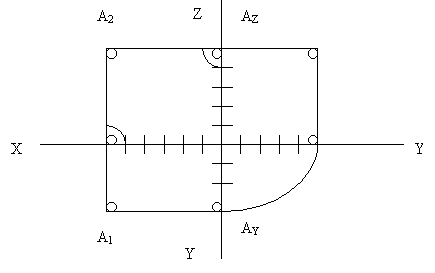
\includegraphics[width=0.48\textwidth]{Images/complexProj}
		\caption{Проекции точки (\rom{1} октант) на комплексном чертеже.}
		\label{fig:complProj}
	
	\end{wrapfigure}
	
Что касается проекций A$_1$ и A$_3$, то и они связаны прямыми A$_1$A$_y$ и A$_3$A$_y$, перпендикулярными оси Y. Но, так как эта ось на эпюре занимает два положения, то отрезок A$_1$A$_y$ не может быть продолжением отрезка A$_3$A$_y$.

Построение проекций точки A на эпюре по заданным координатам выполняют в такой последовательности: прежде всего, на оси абсцисс от начала координат откладывают отрезок OA$_x$ = x, а затем через точку A$_x$ проводят перпендикуляр к оси X, на котором, с учетом знаков, откладываем отрезки A$_x$A$_1$ = y (получаем A$_1$) и A$_x$A$_2$ = z (получаем A$_2$). Остается построить профильную проекцию точки A$_3$. Так как профильная и фронтальная проекции точки должны быть расположены на одном перпендикуляре к оси Z, то через A$_2$ проводят прямую A$_2$A$_z$.

Наконец, возникает последний вопрос: на каком расстоянии от оси Z должна находиться A$_3$? Рассматривая координатный параллелепипед (Рис. \ref{fig:ortSys}), ребра которого A$_z$A$_3$ = OA$_y$ = A$_x$A$_1$ = y, заключаем, что искомое расстояние 
A$_z$A$_3$ равно y. Отрезок A$_z$A$_3$ 
откладывают вправо от оси Z, если y > 0,
 и влево, если y < 0.
 
 \subsection{Структура решения}
 	\begin{enumerate}
 	\item Ввод координат точки пространства и угла между осями координат.
 	\item Перевод трёхмерных координат в координаты экрана. 
 	\begin{itemize}
 		\item Преобразование координат на пространственном чертеже.
 		\item Преобразование координат на комплексном чертеже.
 	\end{itemize}
 	\item Вывод на экран.
 	\begin{itemize}
 		\item Вывод на пространственном чертеже.
 		\item Вывод на комплексном чертеже.
 	\end{itemize}
 	\end{enumerate}
 
\section{Обзор и анализ методов решения}
 \subsection{Ввод координат точки пространства и угла между осями координат.}
 В программе будет реализовано динамическое изменение координат точки и угла между осями. Современные средства разработки приложений содержат в себе стандартные компоненты, с помощью которых можно обеспечить такую функциональность: переключатели (radiobutton), флажки (checkbox), выпадающие списки, ползунковые переключатели. В рамках данной программы наиболее удобным будет использование ползунковых переключателей.
 \\\\
 \emph{Обобщённый алгоритм:}
 	\begin{enumerate}
 		\item Считать значение ползункового переключателя.
 		\item Записать это значение в соответствующую переменную.
 	\end{enumerate}
\subsection{Перевод трёхмерных координат в координаты экрана.}

Для построения чертежей на экране, необходимо перевести координаты из реальной трёхмерной системы координат в двумерную систему координат экрана (для пространственного макета), а также определить по трёхмерных координатам координаты на комплексном чертеже и перевести их в двумерную систему координат экрана.

\subsubsection{Для пространственного чертежа}
Необходимо преобразовать трехмерную систему координат и точку в ней в двумерную систему координат экрана, вычислить координаты проекций точки и линий связи.
Входные данные:	
 	\begin{itemize}
 		\item (x, y, z) - координаты точки в трёхмерном пространстве.
 		\item $\alpha$ - значение угла между отрицательным направлением оси X и положительным направлением оси Y.
 	\end{itemize}
 Выходные данные:	
 	\begin{itemize}
 		\item экранные координаты точек системы координат.
 		\item экранные координаты точки Т(x$_t$,y$_t$)
 		\item экранные координаты точек проекций T$_1$, T$_2$, T$_3$ на плоскости П$_1$, П$_2$ и П$_3$ соответственно.
 		\item экранные координаты точек T$_x$, T$_y$, T$_z$ на осях X, Y и Z соответственно.
 	\end{itemize}
Чтобы изобразить пространственный чертеж, необходимо провести преобразования трёхмерных координат в двумерную систему координат экрана.  (Рис. \ref{fig:screenCoordSys}). \hspace*{\fill}
	\begin{wrapfigure}[13]{h}{0.5\linewidth} 
		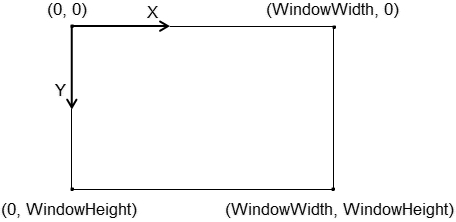
\includegraphics[width=0.48\textwidth]{Images/screenCoordinateSystem}
		\caption{Экранная система координат.}
		\label{fig:screenCoordSys}
	
	\end{wrapfigure}
	
Для удобства пользователя логично расположить начало координат в центре экрана.
Координаты центра вычислим по формулам:
\\
x$_0$ = $\frac{width}{2}$
\\
y$_0$ = $\frac{heigth}{2}$,\\
где \emph{width} и \emph{height} -- ширина и высота экрана соответственно.

Таким образом, нужно вывести формулы для перевода заданных трёхмерных координат произвольной точки T(x, y, z) в двумерные координаты экрана (обозначим их как x$_t$ и y$_t$), учитывая заданный угол между отрицательным направлением оси X и положительным направлением оси Y и заданное выше начало координат.

	\begin{wrapfigure}[19]{r}{0.7\linewidth} 
		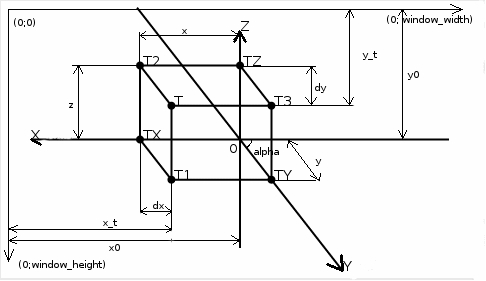
\includegraphics[width=0.67\textwidth]{Images/pointOnCoordinates}
		\caption{}%todo
		\label{fig:pointOnCoords}
	\end{wrapfigure}
	
Из рисунка \ref{fig:pointOnCoords} видно, что:
\\
	x$_t$ = x$_0$ -- x + dx, \\
	y$_t$ = y$_0$ -- z + dy, \\
	dx = y*cos($\alpha$), dy = y*sin($\alpha$)

	Отсюда:
\\
	x$_t$ = x$_0$ -- x + y $\cdot$ cos($\alpha$) (1)\\
	y$_t$ = y$_0$ -- z + y $\cdot$ sin($\alpha$) (2)\\
	
Таким образом, мы получили формулы для вычисления экранных координат произвольной точки трёхмерного пространства по заданным трёхмерным координатам, углу $\alpha$ (углу между отрицательным направлением оси X и положительным направлением оси Y) и началу координат.
	
	Через формулы 1 и 2 мы можем вычислить остальные координаты для пространсвенного чертежа:
	\\
	T$_x$ (x$_0$, y$_0$) \\
	T$_y$ (x$_0$ -- y $\cdot$ cos($\alpha$), y$_0$ + y $\cdot$ sin($\alpha$)) \\
	T$_z$ (x$_0$, y$_0$ -- z)\\
	T$_1$ (x$_0$ -- x + y $\cdot$ cos($\alpha$), y$_0$ + y $\cdot$ sin($\alpha$))\\
	T$_2$ (x$_0$ -- x, y$_0$ -- z)\\
	T$_3$ (x$_0$ + y $\cdot$ cos($\alpha$), y$_0$ -- z + y $\cdot$ sin($\alpha$))\\
	T (x$_0$ -- x + y $\cdot$ cos($\alpha$), y$_0$ -- z + y $\cdot$ sin($\alpha$))
	
	Заметим, что получив координаты точек T$_x$, T$_y$ и  T$_z$ можно использовать эти значения для вычисления точек T, T$_1$, T$_2$ и T$_3$. Таким образом:\\
	T$_1$ (T$_y$ -- x, T$_y$)\\
	T$_2$ (T$_x$, T$_z$)\\
	T$_3$ (T$_y$, T$_y$ -- z)\\
	T (T$_1x$, T$_3y$)
	\\
	
\emph{Обобщенный алгоритм:}
Используя формулы 1, 2, найти:
	\begin{itemize}
		\item экранные координаты начала отсчёта пространственного макета.
		\item экранные координаты точек начала и конца осей системы координат.
		\item экранные координаты точки T.
		\item экранные координаты её проекций на плоскости П$_1$, П$_2$, П$_3$ — точки Т$_1$, Т$_2$ и Т$_3$ соответственно.
		\item экранные координаты её проекций на координатные оси — точки T$_x$, T$_y$, T$_z$.
	\end{itemize}

\subsubsection{Для комплексного чертежа}
Входные данные:
	\begin{itemize}
		\item координаты точки T в трёхмерном пространстве.
	\end{itemize}
	
Выходные данные:
	
	\begin{itemize}
		\item комплексный чертеж.
	\end{itemize}
	
	\begin{wrapfigure}[20]{r!}{0.7\linewidth} 
		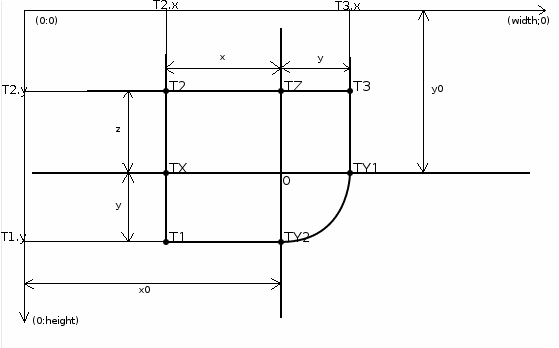
\includegraphics[width=0.67\textwidth]{Images/complexDrawingPrototype}
		\caption{Прототип комплексного чертежа}
		\label{fig:complDrawProto}
	\end{wrapfigure}
	
Центр координат расположим также в центре экрана. Координаты центра находятся как:\\
x$_0$ = $\frac{width}{2}$
\\
y$_0$ = $\frac{heigth}{2}$,\\
где \emph{width} и \emph{height} -- ширина и высота экрана соответстjенно.

Из рисунка \ref{fig:complDrawProto} можно найти координаты всех точек комплексного чертежа:\\
	O (x$_0$, y$_0$) (3)\\
	T$_x$ (x$_0$ -- x, y$_0$) (4)\\
	T$_z$ (x$_0$, y$_0$ -- z) (5)\\
	T$_y1$ (x$_0$ + y, y$_0$) (6)\\
	T$_y2$ (x$_1$, y$_0$ + y) (7)\\
	
Зная координаты точек T$_x$,T$_y1$,T$_y2$ и  T$_z$ можно вычислить значения координат точек  T$_1$, T$_2$ и T$_3$:\\
	T$_1$ (T$_x$.x, T$_y2$.y) \\
	T$_2$ (T$_x$.x, T$_z$.y) \\
	T$_3$ (T$_y1$.x, T$_z$.y) \\
	
\emph{Обобщённый алгоритм:}
Используя формулы 3-7, найти:
	\begin{itemize}
		\item экранные координаты точки начала отсчета комплексного чертежа.
		\item экранные координаты точек начала и конца осей системы координат.
		\item экранные координаты точки T.
		\item Экранные координаты проекций точки Т на плоскости П$_1$, П$_2$ и П$_3$ — точки Т$_1$, Т$_2$ и Т$_3$ соответственно.
		\item Экранные координаты проекций точки Т на оси X, Z и Y — точки T$_x$, T$_z$ и T$_y1$, T$_y2$.
	\end{itemize}
	
\section{Отрисовка (вывод чертежей на экран).}
Для отрисовки чертежей нужно отрисовывать следующие примитивы: линия, окружность и точка. Это можно сделать с помощью стандартных функций.

В \textbf{ОС Windows} для того, чтобы вывести необходимое изображение на устройство вывода (экран, принтер и т. д.) довольно часто используется Интерфейс Графических Устройств GDI (Graphical Device Interface), представляющий собой интерфейс, который Windows использует для рисования 2D графики. Когда приложения обращаются к GDI для вывода графического изображения, они работают не с реальными (физическими) устройствами, а с логическими. Приложения Windows не определяют тип видеомонитора,а работают с логическим видеомонитором. Выполняя запрос приложения, GDI обращается к драйверу соответствующего устройства вывода, а драйвер работает непосредственно с физическим устройством вывода. За счёт этого, в процессе выполнения запроса GDI (или драйвер) учитывает ограниченные возможности физического устройства вывода и его аппаратные особенности, делая необходимые приближения. 

В \textbf{UNIX-подобных} системах для вывода графики почти повсеместно используется X Window System. Она берет на себя заботы о вводе и выводе на низком уровне, предоставляя пользовательским программам работать в терминах оконного интерфейса. X Window System использует традиционную оконную модель, в которой пространством ресурсов является экран. Экран — это прямоугольник, на котором отображаются команды графического вывода и организуется обратная связь с устройствами графического ввода. Программа, которая отвечает за работу с устройствами графического ввода и вывода и обеспечивает при этом логику оконной системы, называется X-сервером. В рамках X Window System, X-сервер — это ядро. Он выполняет низкоуровневые операции и взаимодействует с аппаратурой, ничего самостоятельно не предпринимая. Подобно ядру, он предоставляет задачам унифицированный интерфейс к этим низкоуровневым функциям, а также занимается разделением доступа (окно и фокус) к графическим ресурсам. X-сервер не волнует, отчего эти задачи вообще появляются и чем живут. Он только принимает запросы на выполнение графических действий и передаёт по назначению вводимые данные. Жизнеобеспечение процессов и даже способ передачи X-запросов — дело исключительно операционной системы, по отношению к которой и сам X-сервер — задача.

Задачи, которые обращаются к X-серверу с запросами, называются X-клиентами. Обычно X-клиент сначала регистрирует окно (можно несколько), которое и будет ему полем ввода-вывода. Потом он сможет рисовать в этом окне и обрабатывать происходящие с окном события: активность устройств ввода и изменение свойств самого окна (размер, перемещение, превращение в иконку, закрытие и т. п.). X-клиент в Linux — это процесс, запускаемый обычно в фоне не связанный по вводу с терминальной линией). 

Таким образом, нам необходимо, чтобы наш фреймворк умел обращаться к API выбранной нами ОС и предоставлял нам высокоуровневый интерфейс для отрисовки линий, окружностей и точек в виде структур Line, Circle и Point соответсвенно.

%\subsection{Обобщённый алгоритм}

\subsection{Описание и реализация применяемых методов}
Координаты точек и функции по вычислению их значения выделены в структуры \textbf{DimensionalDrawing} для пространственного чертежа и \textbf{ComplexDrawing} для комплексного чертежа. Координаты двумерных точек хранятся в виде структур Point, атрибутами которого являются значения x и y, точка T хранится как структура Point3, с атрибутами x, y и z. Координаты отрезков хранятся в структурах типа Line, с атрибутами p1 и p2, представляющими из себя структуры типа Point. Две константы,\\ COMPLEX\_BACKGROUND\_COLOR и \ DIMENSIOANL\_BACKGROUND\_COLOR отвечают за цвета фона комплексного и пространственного чертежей соответсвенно; за цвета точек отвечает константа POINT\_COLOR. Константа BRUCH\_SIZE хранит информацию о том, какой толщины будут линии отрисовываемых фигур.

\subsubsection{Ввод координат точки пространства и угла между осями}
Для ввода координат и угла между осями используются виджеты типа <<ползунковый переключатель>>. Для каждого из них определяется диапазон значений и значение инкремента.

Считывание значений из <<ползунковых переключателей>> и запись этих значений в переменные происходит следующим образом:
\lstset {language=C++}
\begin{lstlisting}
x = sliderX.value
y = sliderY.value
z = sliderZ.value
Point3 coordinates = (x, y, z)
alpha = sliderAlpha.value()
\end{lstlisting}

\subsubsection{Вычисления. Укрупненный алгоритм}
\emph{Для пространственного чертежа}:

Необходимо преобразовать трехмерную систему координат и точку в ней в двумерную систему координат экрана, вычислить координаты проекций точки и линий связи.

	\begin{itemize}
		\item width -- ширина области чертежа.
		\item height — высота области чертежа.
		\item O (x$_0$, y$_0$) -- точка начала координат.
		\item angle -- угол между положительным направлением оси Y и отрицательным направлением оси X.
		\item OX\_begin, OX\_end, OY\_begin, OY\_end, OZ\_begin, OZ\_end — начальные и конечные точки осей координат.
		\item x, y, z -- координаты точки Т в трёхмерном пространстве.
	\end{itemize}
	
\textbf{Алгоритм:}

Используя формулы 1, 2, найдем:

	\begin{itemize}
		\item Экранные координаты начальных и конечных точек осей X, Y и Z.
T(x$_0$, y$_0$) (2) — точка начала координат, OX\_begin(x,y), OX\_end(x,y) -- крайние точки оси X, OY\_begin(x,y), OY\_end(x,y) -- крайние точки оси Y. OZ\_begin(x,y), OZ\_end(x,y) -- крайние точки оси Z.
		\item Экранные координаты проекций точки Т на координатные оси.\\
Т$_x$ (x, y) -- проекция на ось X.\\
T$_y$ (x, y) -- проекция на ось Y.\\
T$_z$ (x, y) -- проекция на ось Z.\\
		\item Экранные координаты точки T. T(X$_t$, Y$_t$)
		\item Экранные координаты проекций точки Т на плоскости П$_1$, П$_2$ и П$_3$.\\
T$_1$ (x,y) -- проекция на плоскость П$_1$.\\
T$_2$ (x,y) -- проекция на плоскость П$_2$.\\
Т$_3$ (x,y) -- проекция на плоскость П$_3$.

	\end{itemize}
	
	\emph{Для комплексного чертежа:}
	
	\begin{itemize}
		\item width -- ширина чертежа.
		\item height -- высота чертежа.
		\item indent -- отступ от границы чертежа.  

	\end{itemize}
	
\textbf{Алгоритм:}

Используя формулы 3-7, найдем:
	\begin{itemize}
		\item Экранные координаты центра координат.\\
O (x$_0$,y$_0$) -- центр координат
		\item Экранные координаты начальных и конечных точек осей XY и ZY.
	XY\_begin(x,y), XY\_end(x,y) -- крайние точки оси XY.
	ZY\_begin(x,y), ZY\_end(x,y) -- крайние точки оси ZY.
		\item Экранные координаты проекций точки Т на координатные оси.\\
	T$_x$ (x, y) -- проекция на ось X.\\
	T$_z$ (x, y) -- проекция на ось Z.\\
	T$_y1$ (x, y) -- проекция на ось Y.\\
	T$_y2$ (x, y) -- проекция на ось Y.  
		\item Экранные координаты проекций точки Т на плоскости П$_1$, П$_2$ и П$_3$.\\
	T$_1$ (x, y) — проекция на плоскость П$_1$.\\
	Т$_2$ (x, y) — проекция на плоскость П$_2$.\\
	Т$_3$ (x, y) — проекция на плоскость П$_3$.\\
	\end{itemize}
	
	
\subsection{Прорисовка. Укрупненный алгоритм}
\subsubsection{Отрисовка пространственного чертежа. Укрупненный алгоритм}
\textbf{Прорисовка осей}

Чтобы нарисовать оси системы координат, необходимо соединить линиями точки OX\_begin -- OX\_end, OY\_begin -- OY\_end, OZ\_begin -- OZ\_end. Отрисовка оси производится с помощью функции drawLine(). Подпись осей с помощью функции drawText().\\
\\
\textbf{Прорисовка точек}

Точки Т, Т$_1$, Т$_2$, Т$_3$, T$_x$, T$_y$, T$_z$ отрисовываются с помощью функции drawEllipce(). Подпись точек производится с помощью функции drawText().\\
\\
\textbf{Прорисовка линий связи}

Чтобы отрисовать линии связи, необходимо соединить линиями точки T$_1$-T$_x$, T$_1$,-T, T-T$_2$, T$_2$-T$_x$, T$_2$-T$_z$, T-T$_3$, T$_1$-T$_y$, T$_z$-T$_3$, T$_3$-T$_y$. Линии рисуются с помощью функции drawLine().

\subsubsection{Отрисовка комплексного чертежа. Укрупненный алгоритм}
\textbf{Прорисовка осей}

Чтобы нарисовать оси, наобходимо соединить линиями точки XY\_begin -- XY\_end и ZY\_begin -- ZY\_end. Отрисовка оси производится с помощью функции drawLine(). Подпись осей с помощью функции drawText().\\
\\
\textbf{Прорисовка точек}

Точки T$_1$, T$_2$, T$_3$, T$_x$, T$_y1$, T$_y2$, T$_z$ отрисовываются с помощью функции drawEllipce(). Подпись точек производится с помошью функции drawText().\\
\\
\textbf{Прорисовка линий связи}

Чтобы отрисовать линии связи необходимо соединить линиями точки T$_y1$-T$_1$, T$_1$-T$_x$, T$_x$-T$_2$, T$_2$-T$_z$, T$_z$-T$_3$, T$_3$-T$_y1$ и отрисовать дугу T$_y1$-T$_y2$. Линии отрисовываются с помощью функции QPainter::drawLine(), а дуга -- функцией drawArc().

\subsection{Вычисления. Детализированный алгоритм}
\subsubsection{Пространственный чертеж}

Разобём задачу перевода координат в координаты экрана на две части -- сначала, в контроллере, вычислим проекцию точки на плоскость, а затем, в виджете пространственного чертежа, перенесём получившиеся координаты в координаты относительно точки О.

\emph{Функция для вычисления значения точки в координатах экрана:}
\lstset {language=C++}
\begin{lstlisting}
Point point(x, y, z, alpha){
    x = x - y * cos(alpha * PI/180);
    y = z - y * sin(alpha * PI/180);
    return Point(-x, y);
}
\end{lstlisting}
\emph{Перевод координат точки в координаты относительно точки О:}
\begin{lstlisting}
Point ranslateToNativeCoords(Point p){
    p.setY(-p.y);
    p += Point(width / 2, height / 2);
}
\end{lstlisting}
\emph{Перевод координат линии в координаты относительно точки O:}
\begin{lstlisting}
Line translateToNativeCoords(Line l){

    Point p1 = l.p1;
    Point p2 = l.p2;

    tempY = p1.y;

    p1.setY(p2.y);
    p2.setY(tempY);

    l.setPoints(p1, p2);
    l.translate(width / 2, height / 2);
}
\end{lstlisting}

Координаты вспомогательных точек Т$_1$, Т$_2$, Т$_3$, T$_x$, T$_y$, T$_z$ вычисляются в функции:
\begin{lstlisting}
Points dimensionalDravingPoints(x, y, z, alpha){
    Point tx, ty, tz, xy, yz, xz;
    
    tx = Point(- x, 0);
    tz = Point(0, z);
    ty = Point(
                y * cos(alpha * PI/180),
               -y * sin(alpha * PI/180)
                );

    xz = Point(-x, z);

    yz = Point(
                y * cos(alpha * PI/180),
                z - y * sin(alpha * PI/180)
                );
    xy = Point(
                - (x - y * cos(alpha * PI/180)),
                -y * sin(alpha * PI/180)
                );

    Points points = {
        {"Tx", tx},
        {"Ty", ty},
        {"Tz", tz},
        {"Txy", xy},
        {"Txz", xz},
        {"Tyz", yz}
    };

    return points;
}
\end{lstlisting}
Эти точки также переводятся в координаты чертежа с помощью функции
\\
<<translateToNativeCoords(Point)>>.

\subsubsection{Комплексный чертеж}
Разобём задачу перевода координат в координаты экрана на две части -- сначала, в контроллере, вычислим значение точки в координатах экрана, а затем, в виджете пространственного чертежа, перенесём эти координаты в координаты относительно точки О.

\emph{Функция для вычисления значения точкек  точек T, Т$_1$, Т$_2$, Т$_3$, T$_x$, T$_y$, T$_z$ в координатах экрана:}
\lstset {language=C++}
\begin{lstlisting}
Points complexDravingPoints(x, y, z){
    Point tx, ty1, ty2, tz, t1, t2, t3;

    tx = Point(-x, 0);

    tz = Point(0, z);

    ty1 = Point(y, 0);
    ty2 = Point(0, y);

    t1 = Point(tx.x, ty2.y);
    t2 = Point(tx.x(), tz.y);
    t3 = Point(ty1.x, tz.y);

    Points points = {
        {"T1", t1},
        {"T2", t2},
        {"T3", t3},
        {"Tx", tx},
        {"Tz", tz},
        {"Ty1", ty1},
        {"Ty2", ty2}
    };
    return points;
}
\end{lstlisting}
\emph{Перевод координат точки в координаты относительно точки О:}
\begin{lstlisting}
Point translateToNativeCoords(Point p){
    p.setY(-p.y());
    p += Point(width / 2, height / 2);
}
\end{lstlisting}
\emph{Перевод координат линии в координаты относительно точки O:}
\begin{lstlisting}
Line translateToNativeCoords(Line l){

    Point p1 = l.p1;
    Point p2 = l.p2;

    tempY = p1.y;

    p1.setY(p2.y);
    p2.setY(tempY);

    l.setPoints(p1, p2);
    l.translate(width / 2, height / 2);
    return l;
}
\end{lstlisting}
\subsection{Прорисовка. Детализированный алгоритм}
\subsubsection{Пространственный чертеж}
Прорисовка происходит в функции:
\begin{lstlisting}
paintEvent(){
    Painter paint(this);

    Font font;
    font.setFamily("Arial");
    font.setPointSize(11);

    paint.setFont(font);
    Pen pen;
    Brush brush(COMPLEX_BACKGROUND_COLOR);
    paint.setBrush(brush);
    paint.drawRect(0,0, width, height);

    pen.setColor(QColor(0,0,0,255));
    paint.setPen(pen);

    Line x = _coordinateAxes.value("X");
    this->translateToNativeCoords(x);
    paint.drawLine(x);
    paint.drawText(x.p1(), "X");

    Line y = _coordinateAxes.value("Y");
    this->translateToNativeCoords(y);
    paint.drawLine(y);
    paint.drawText(y.p1(), "Y");

    Line z = _coordinateAxes.value("Z");
    this->translateToNativeCoords(z);
    paint.drawLine(z);
    paint.drawText(z.p1(), "Z");

    Point t = _point;
    this->translateToNativeCoords(t);

    paint.drawText(t, "T");

    Point zero(0,0);
    this->translateToNativeCoords(zero);
    paint.drawEllipse(zero, 2, 2);
    zero += QPoint(10, -10);
    paint.drawText(zero, "0");

    pen.setColor(Qt::blue);
    brush.setColor(Qt::blue);
    paint.setPen(pen);
    paint.setBrush(brush);
    Point tx, ty, tz, xy, xz, yz;
    tx = _helperPoints.value("Tx");
    ty = _helperPoints.value("Ty");
    tz = _helperPoints.value("Tz");

    xy = _helperPoints.value("Txy");
    xz = _helperPoints.value("Txz");
    yz = _helperPoints.value("Tyz");

    foreash(p in _helperPoints){
        paint.drawEllipse(p, 2, 2);
    }

    paint.drawEllipse(t, 2, 2);

    pen.setColor(black);
    brush.setColor(black);
    paint.setPen(pen);
    paint.setBrush(brush);

    font.setPointSize(9);
    paint.setFont(font);

    Point p;
    foreash(p in helperPoints.keys()){
        p = _helperPoints.value(k);
        paint.drawText(p, k);
    }

    pen.setStyle(Qt::DashLine);
    pen.setColor(QColor(115, 117, 115, 255));
    paint.setPen(pen);

    paint.drawLine(t, xz);
    paint.drawLine(t, yz);
    paint.drawLine(t, xy);

    paint.drawLine(tx, xy);
    paint.drawLine(tx, xz);

    paint.drawLine(ty, yz);
    paint.drawLine(ty, xy);

    paint.drawLine(tz, xz);
    paint.drawLine(tz, yz);

}
\end{lstlisting}
\subsubsection{Комплексный чертеж}
Прорисовка происходит в функции:
\begin{lstlisting}
void paintEvent(){
    QPainter paint(this);
    QPen pen;
    QBrush brush(DIMENSIONAL_BACKGROUND_COLOR);
    paint.setBrush(brush);
    paint.drawRect(0,0,width, height);

    int size = this->width / 2 - 20;
    Line x, y;
    y.setP1(Point(0, size));
    y.setP2(Point(0, -size));

    x.setP1(Point( -size, 0));
    x.setP2(Point(size, 0));

    translateToNativeCoords(x);
    translateToNativeCoords(y);

    paint.drawLine(x);
    paint.drawLine(y);
    paint.drawText(y.p1, "Z");
    paint.drawText(x.p1, "X");
    paint.drawText(x.p2, "Y");
    paint.drawText(y.p2, "Y");

    foreash(p in _points){
        ranslateToNativeCoords(p);
        paint.drawEllipse(p, 2, 2);
    }

    Point t1 = _points.value("T1");
    paint.drawText(t1, "T1");

    Point t2 = _points.value("T2");
    paint.drawText(t2, "T2");

    Point t3 = _points.value("T3");
    paint.drawText(t3, "T3");

    Line line(t1, t2);
    paint.drawLine(line);

    line.setPoints(t2,t3);
    paint.drawLine(line);

    Point zero(0,0);
    this->translateToNativeCoords(zero);
    paint.drawEllipse(zero, 1, 1);

    Point ty1 = _points.value("Ty1");
    Point ty2 = _points.value("Ty2");

    int delta = ty1.x() - zero.x();

    Point areaPoint(zero.x() - delta, zero.y() - delta);

    int startAngle = zero.x() > ty1.x() ? 90*16 : 0;
    int spainAngle = zero.x() > ty1.x() ? 90*16 : -90*16;

    paint.drawArc(QRect(areaPoint, area), 
    			startAngle, spainAngle);

    zero += Point(10, -10);
    paint.drawText(zero, "0");

    pen.setStyle(DashLine);
    paint.setPen(pen);

    paint.drawLine(t1, ty2);
    paint.drawLine(t3, ty1);

}

\end{lstlisting}
\section{Руководство программиста}
Программа написана на языке C++14 с использованием кроссплатформенной библиотеки Qt. Изображения выводятся на виджетах, унаследованных от класса QWidget: это ComplexDrawing и DimensionalDrawing для комплексного и пространственного чертежей соответственно. Ввод данных осуществляется с помощью ползунковых переключателей типа QSlider. Для отображения текста используется виджет QLabel.
\\\\
Виджеты QSlider:
\begin{itemize}
	\item sliderX -- изменяет координату x.
	\item sliderY -- изменяет координату y.
	\item sliderZ -- изменяет координату z.
	\item sliderAlpha -- изменяет угол $\alpha$.
\end{itemize}

Функция \emph{QSlider::value()} возвращает значение, на котором сейчас установлен QSlider.

Для передачи значений точек от класса Controller классам ComplexDrawing и DimensionalDrawing используется QHash<QString, QPoint>, который является стандартной реализацией словаря типа ключ-значение.
\subsection{Функциональная схема программы (Рис. \ref{fig:classDyagr})}

	\begin{figure}[h]
		\center{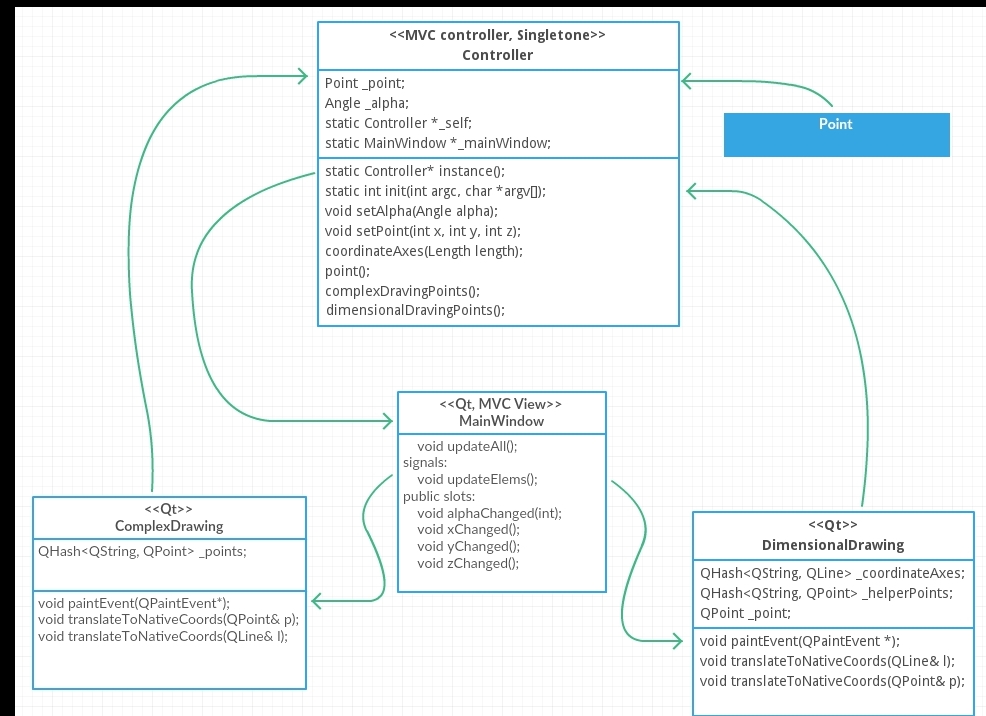
\includegraphics[width=\textwidth]{Images/classDyagram}}
		\caption{Функциональная схема программы}
		\label{fig:classDyagr}
	
	\end{figure}
	
В программе используется пять классов:
\begin{enumerate}
	\item Point -- класс, хранящий координаты 3D точки. В нем имеются только 3 атрибута:
		\begin{itemize}
			\item x -- координата по оси x
			\item y -- координата по оси y
			\item z -- координата по оси z
		\end{itemize}
	\item MainWindow --  класс, реализующий основную форму программы. В нем происходит инициализация других виджетов и установка их параметров.
	\item DimensionalDrawing -- класс, описывающий пространственный чертеж. Хранит информацию о всех точках пространсвенного чертежа и линиях координат.
	\item ComplexDrawing -- класс, описывающий комплексный чертеж. Хранит информацию о всех точках комплексного чертежа и линиях координат. 
	\item Controller -- класс, инициализирующий MainWindow, хранящий информацию о координатах точки (в экземпляре класса Point). Controller реализует методы пересчета координат точек для пространственного и комплексного чертежей.
\end{enumerate}

При запуске программы создаётся экземпляр класса Controller, котрый создаёт экземпляр класса MainWindow:
\begin{lstlisting}

int Controller::init(int argc, char *argv[]){
    QApplication a(argc, argv);
    Controller::_mainWindow = new MainWindow();
    _mainWindow->show();
    return a.exec();
}
\end{lstlisting}

При изменении значения в каком либо из ползунковых переключателей, происходит вызов функции контроллера, изменяет пересчитывает координаты нужных точек и вызывает перерисовку виджетов DimensionalDrawing и ComplexDrawing:
\begin{lstlisting}
void Controller::setPoint(int x, int y, int z){
    _point = Point(x, y, z);
    _mainWindow->updateAll();
}
\end{lstlisting}
После этого, классы DimensionalDrawing и ComplexDrawing вызывают функции контроллера для получения пересчитанных точек, переводят их в свои относительные координаты и отрисовывают:

\begin{lstlisting}
void ComplexDrawing::updateElems(){
    _points = Controller::instance()->complexDravingPoints();
    for(auto&x : _points){
        this->translateToNativeCoords(x);
    }
    update();
}
\end{lstlisting}
\begin{lstlisting}
void DimensionalDrawing::updateElems(){
    _coordinateAxes = Controller::instance()->coordinateAxes(this->width() / 2 - 20);
    _point = Controller::instance()->point();
    _helperPoints = Controller::instance()->dimensionalDravingPoints();

    for(auto&x : _helperPoints){
        this->translateToNativeCoords(x);
    }

    update();
}
\end{lstlisting}

В этих функциях происходит вызов функций контроллера \emph{complexDravingPoints()} и \emph{dimensionalDravingPoints()}, которые отвечают за перевод трехмерной системы в координаты экрана:
\begin{lstlisting}
QHash<QString, QPoint> Controller::complexDravingPoints(){
    QPoint tx, ty1, ty2, tz, t1, t2, t3;
    tx = QPoint(- _point.x(), 0);
    tz = QPoint(0, _point.z());
    ty1 = QPoint(_point.y(), 0);
    ty2 = QPoint(0, -_point.y());
    t1 = QPoint(tx.x(), ty2.y());
    t2 = QPoint(tx.x(), tz.y());
    t3 = QPoint(ty1.x(), tz.y());
    QHash<QString, QPoint> points = {
        {"T1", t1},
        {"T2", t2},
        {"T3", t3},
        {"Tx", tx},
        {"Tz", tz},
        {"Ty1", ty1},
        {"Ty2", ty2}
    };
    return points;
}

QHash<QString, QPoint> Controller::dimensionalDravingPoints(){
    QPoint tx, ty, tz, xy, yz, xz;

    tx = QPoint(0,0);
    ty = QPoint(0,0);
    tz = QPoint(0,0);
    xz = QPoint(0,0);
    yz = QPoint(0,0);
    xy = QPoint(0,0);

    tx = QPoint(- _point.x(), 0);
    tz = QPoint(0, _point.z());
    ty = QPoint(
                _point.y() * cos(_alpha * M_PI/180),
               -_point.y() * sin(_alpha * M_PI/180)
                );

    xz = QPoint(-_point.x(), _point.z());

    yz = QPoint(
                _point.y() * cos(_alpha * M_PI/180),
                _point.z() - _point.y() * sin(_alpha * M_PI/180)
                );
    xy = QPoint(
                - (_point.x() - _point.y() * cos(_alpha * M_PI/180)),
                -_point.y() * sin(_alpha * M_PI/180)
                );

    QHash<QString, QPoint> points = {
        {"Tx", tx},
        {"Ty", ty},
        {"Tz", tz},
        {"Txy", xy},
        {"Txz", xz},
        {"Tyz", yz}
    };

    return points;
}
\end{lstlisting}
\section{Руководство пользователя}
	\begin{figure}[h]
		\center{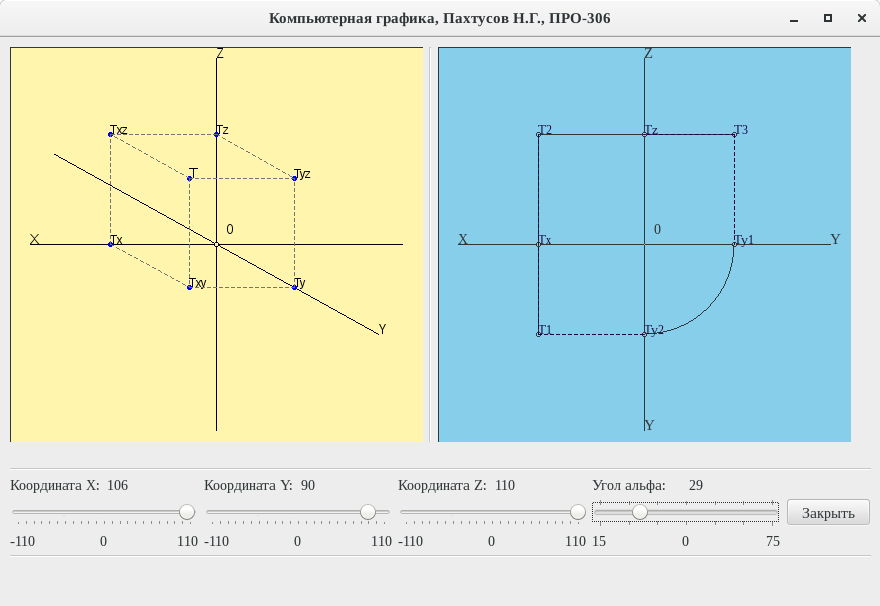
\includegraphics[width=\textwidth]{Images/ApplicationScreen}}
		\caption{Вид приложения}
		\label{fig:appScr}
	
	\end{figure}
После запуска программы пользователь видит в окне программы два поля: в левом рисуется пространственный чертеж, а в правом -- комплексный чертеж. Изменяя положение ползунков в нижней части окна, пользователь может изменять координаты точки в пространстве и угол между отрицательным направлением оси X и положительным направлением оси Y. Окно приложения представленно на Рис. \ref{fig:appScr}.

\section{Заключение}
В ходе данной лабораторной работы были выведены формулы для расчёта экранных координат точки трёхмерного пространства для построения пространственного и комплексного чертежей. Была разработана программа, выводящая на экран пространственный и комплексный чертежи и позволяющая динамически изменять координаты точки и угол между осями X и Y.
 \end{document}
